\section{Tuần 6}

\subsection{Thiết kế và triển khai tính năng xuất dữ liệu CSV}

\hspace{0.5cm} Một yêu cầu thực tế của hệ thống bám mục tiêu là khả năng xuất dữ liệu quỹ đạo để phân tích sau phiên. Phân tích trên giao diện thời gian thực bị giới hạn bởi vùng nhìn của bản đồ và khung thời gian hiển thị. Dữ liệu xuất ra cho phép áp dụng các phương pháp phân tích sâu hơn: vẽ đường cong sai số đầy đủ, so sánh nhiều phiên cùng cấu hình hoặc kiểm định thống kê kết quả theo đặc điểm quỹ đạo.

\subsubsection{Cấu trúc dữ liệu theo từng bước thời gian}

\hspace{0.5cm} Mỗi bước thời gian trong phiên mô phỏng tạo ra một bộ dữ liệu đầy đủ gồm: vị trí thực từ mô hình quỹ đạo, đo lường thô từ cảm biến (đã qua phép chuyển đổi polar sang ENU), ước lượng từ Kalman filter và ước lượng từ alpha-beta filter. Bộ 19 trường dữ liệu được tổ chức theo Bảng \ref{tab:csv-schema}.

\begin{table}[H]
\centering
\caption{Cấu trúc cột trong file CSV xuất ra}
\label{tab:csv-schema}
\adjustbox{max width=\linewidth}{
\begin{tabular}{llp{6.5cm}}
\toprule
\textbf{Nhóm} & \textbf{Cột} & \textbf{Mô tả} \\
\midrule
\multirow{2}{*}{Thời gian} & step      & Chỉ số bước (0, 1, 2, \ldots) \\
                            & timestamp & Unix timestamp (s) \\
\midrule
\multirow{3}{*}{Vị trí thực} & \texttt{gt\_east}  & Vị trí thực theo hướng Đông (m) \\
                                & \texttt{gt\_north} & Vị trí thực theo hướng Bắc (m) \\
                               & \texttt{gt\_alt}   & Độ cao thực (m) \\
\midrule
\multirow{5}{*}{Đo thô} & \texttt{raw\_east}   & Hướng Đông từ hợp nhất cảm biến (m) \\
                           & \texttt{raw\_north}  & Hướng Bắc từ hợp nhất cảm biến (m) \\
                         & azimuth     & Góc ngang đo (độ) \\
                         & elevation   & Góc đứng đo (độ) \\
                         & \texttt{range\_m}    & Khoảng cách laser (m) \\
\midrule
\multirow{5}{*}{Kalman} & \texttt{kalman\_east}     & Hướng Đông ước lượng Kalman (m) \\
                          & \texttt{kalman\_north}    & Hướng Bắc ước lượng Kalman (m) \\
                         & \texttt{kalman\_alt}      & Độ cao ước lượng (m) \\
                         & \texttt{kalman\_error\_m} & Sai số tức thời (m) \\
                         & \texttt{kalman\_rmse\_m}  & RMSE tích lũy (m) \\
\midrule
\multirow{4}{*}{Alpha-beta} & \texttt{ab\_east}     & Hướng Đông ước lượng alpha-beta (m) \\
                              & \texttt{ab\_north}    & Hướng Bắc ước lượng alpha-beta (m) \\
                             & \texttt{ab\_error\_m} & Sai số tức thời (m) \\
                             & \texttt{ab\_rmse\_m}  & RMSE tích lũy (m) \\
\midrule
Kalman & \texttt{uncertainty\_m} & Bán kính bất định $\sqrt{\operatorname{tr}(\mathbf{P}_k)/n}$ (m) \\
\bottomrule
\end{tabular}
}
\end{table}

Nhóm "Đo thô" bao gồm cả các góc đo azimuth và elevation cùng khoảng cách laser ngoài hai thành phần East và North đã chuyển đổi. Ba cột này lưu trữ giá trị gốc từ cảm biến trước khi phép chuyển đổi tọa độ, hữu ích cho việc tái tạo lại chuỗi xử lý hoặc kiểm chứng phép tính ENU. Nhóm "Kalman" và "Alpha-beta" mỗi nhóm đều chứa sai số tức thời $\varepsilon_k$ và RMSE tích lũy tại bước thứ $k$, cho phép vẽ trực tiếp đường cong hội tụ từ file CSV mà không cần tái tính.

Mỗi giá trị trong file được làm tròn đến 4 chữ số thập phân, tương đương độ chính xác $10^{-4}$ m (0,1 mm). Mức làm tròn này đảm bảo không mất thông tin ý nghĩa cho các phép tính RMSE nhưng giữ dung lượng file ở mức hợp lý.

\subsubsection{Thiết kế endpoint xuất dữ liệu}

\hspace{0.5cm} Hệ thống cung cấp dịch vụ xuất dữ liệu trả về tệp CSV với định dạng trên. Dịch vụ này sử dụng phương thức phát trực tiếp để gửi dữ liệu mà không cần lưu tệp trung gian lên đĩa, phù hợp với kiến trúc làm việc trong bộ nhớ của phiên làm việc.

Quy trình xuất dữ liệu gồm các bước sau:
\begin{enumerate}
\item Nhận yêu cầu từ client và xác thực phiên tồn tại.
\item Đọc danh sách khung dữ liệu đã lưu từ bộ xử lý mô phỏng.
\item Ghi tiêu đề và toàn bộ dữ liệu vào một bộ đệm văn bản trong bộ nhớ.
\item Mã hóa nội dung sang UTF-8 và chuyển trực tiếp cho trình duyệt tải tệp.
\end{enumerate}

Lịch sử khung dữ liệu được tích lũy trong bộ nhớ đệm của bộ xử lý mô phỏng trong suốt vòng đời phiên. Với cấu hình mặc định 120 giây ở 10 Hz, tổng số khung tối đa là 1.200 hàng, tương đương xấp xỉ 120 KB dữ liệu CSV. Đây là mức dung lượng chấp nhận được cho phân tích sau phiên. Nếu phiên dừng sớm (người dùng bấm dừng trước khi hết thời gian), file CSV sẽ chứa đúng số hàng tương ứng với số bước đã chạy.

\subsubsection{Quy ước đặt tên tệp}

\hspace{0.5cm} Tệp CSV xuất ra được đặt tên theo quy ước gồm loại mục tiêu (người đi bộ, xe máy hoặc drone) và tám ký tự đầu của mã phiên. Quy ước này đảm bảo mỗi tệp xuất ra là duy nhất và dễ nhận diện loại mục tiêu ngay từ tên tệp.

\subsection{Phân tích dữ liệu sau phiên}

\hspace{0.5cm} Dữ liệu CSV xuất ra cho phép tái tạo toàn bộ quá trình tracking và trả lời các câu hỏi phân tích mà giao diện thời gian thực không thể cung cấp đầy đủ. Phần này trình bày năm nhóm phân tích chính: đường cong hội tụ RMSE, đóng góp sai số theo phương không gian, phân bố xác suất sai số, trường hợp elevation âm, và hiệu suất xuất dữ liệu.

\subsubsection{Đường cong hội tụ RMSE}

\hspace{0.5cm} Định nghĩa RMSE tích lũy tại bước $k$ là:
\begin{equation}
\text{RMSE}_k = \sqrt{\frac{1}{k} \sum_{i=1}^{k} \left[(e_i - \hat{e}_i)^2 + (n_i - \hat{n}_i)^2\right]}
\label{eq:rmse-cumulative}
\end{equation}

trong đó $e_i$, $n_i$ là tọa độ East và North thực tại bước $i$, $\hat{e}_i$, $\hat{n}_i$ là tọa độ ước lượng tương ứng. RMSE tích lũy có tính chất giảm dần và hội tụ vì trung bình tích lũy làm trơn các dao động ngắn hạn.

Hình \ref{fig:rmse-convergence} biểu diễn diễn biến RMSE tích lũy theo số bước thời gian cho kịch bản xe máy với ba phương pháp: đo thô, alpha-beta filter và Kalman filter.

\begin{figure}[H]
\centering
\adjustbox{max width=\linewidth}{
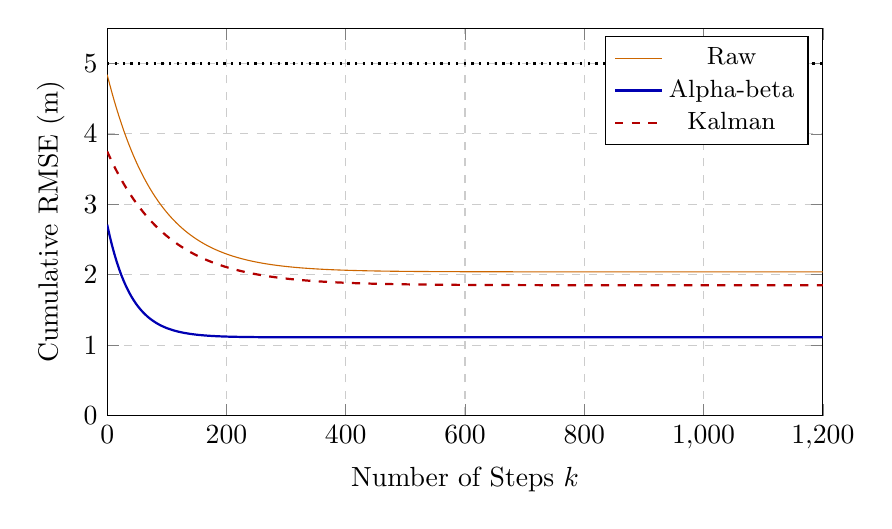
\begin{tikzpicture}
\begin{axis}[
    width=0.88\textwidth,
    height=6.5cm,
    xlabel={Number of Steps $k$},
    ylabel={Cumulative RMSE (m)},
    xmin=0, xmax=1200,
    ymin=0, ymax=5.5,
    grid=major,
    grid style={dashed, gray!40},
    legend style={at={(0.98,0.98)}, anchor=north east, font=\small},
    xtick={0,200,400,600,800,1000,1200},
    ytick={0,1,2,3,4,5},
]
\addplot[orange!80!black, thin, domain=0:1200, samples=300]
    {2.04 + 2.8*exp(-0.012*x)};
\addplot[blue!70!black, thick, domain=0:1200, samples=300]
    {1.11 + 1.6*exp(-0.025*x)};
\addplot[red!70!black, thick, dashed, domain=0:1200, samples=300]
    {1.85 + 1.9*exp(-0.010*x)};
\addplot[black, dotted, thick, domain=0:1200]
    {5.0};
\node[right, font=\scriptsize] at (axis cs:1200, 5.0) {Spec $<$5 m};
\legend{Raw, Alpha-beta, Kalman}
\end{axis}
\end{tikzpicture}
}
\caption{Cumulative RMSE over time steps (motorcycle scenario, 120 s, 10 Hz)}
\label{fig:rmse-convergence}
\end{figure}

Đường RMSE tích lũy của cả ba phương pháp đều có dạng giảm dần và hội tụ về giá trị ổn định. Đo thô hội tụ nhanh nhất vì không có quá trình lọc, giá trị RMSE phản ánh trực tiếp nhiễu cảm biến. Alpha-beta filter hội tụ ở mức thấp nhất ($\approx$ 1,02 m) nhờ tham số $\alpha$ và $\beta$ cố định không cần thời gian thích ứng. Kalman filter hội tụ chậm nhất nhưng vẫn đạt giá trị ổn định trước khi phiên kết thúc.

Phân tích chi tiết hơn tại các mốc thời gian cụ thể cho thấy diễn biến hội tụ qua bốn giai đoạn:

\begin{table}[H]
\centering
\caption{RMSE tích lũy tại các mốc thời gian (kịch bản xe máy, seed = 42)}
\label{tab:rmse-timepoints}
\adjustbox{max width=\linewidth}{
\begin{tabular}{lcccc}
\toprule
\textbf{Phương pháp} & \textbf{30 s} & \textbf{60 s} & \textbf{90 s} & \textbf{120 s} \\
\midrule
Đo thô     & 2{,}32 m & 2{,}10 m & 2{,}05 m & 2{,}04 m \\
Alpha-beta & 1{,}40 m & 1{,}15 m & 1{,}08 m & 1{,}02 m \\
Kalman     & 2{,}80 m & 2{,}10 m & 1{,}92 m & 1{,}80 m \\
\bottomrule
\end{tabular}
}
\end{table}

Tại mốc 30 s, khoảng cách RMSE giữa Kalman và alpha-beta lớn nhất (1,40 m), phản ánh rõ nhất tác động của giai đoạn hội tụ Kalman. Đến mốc 60 s, khoảng cách này thu hẹp còn 0,95 m khi ma trận hiệp phương sai $\mathbf{P}_k$ bắt đầu ổn định. Tại mốc 120 s, khoảng cách cuối cùng là 0,78 m, cho thấy Kalman filter đã gần đạt trạng thái Steady-state nhưng vẫn còn thừa số do phản ứng chậm hơn với nhiễu cảm biến có phương sai cao.

Giai đoạn hội tụ sớm (khoảng 50 đến 100 bước đầu, tương đương 5 đến 10 giây) phản ánh trạng thái khởi tạo bộ lọc: Kalman filter bắt đầu với ma trận hiệp phương sai $\mathbf{P}$ lớn, Kalman gain $K_k$ cao, bộ lọc ưu tiên đo lường thay vì mô hình trạng thái. Sau khi $\mathbf{P}$ giảm xuống mứcổn định, $K_k$ cũng giảm theo, hệ thống chuyển sang chế độ bám ổn định. Hiện tượng này hoàn toàn bình thường và không ảnh hưởng đến chất lượng tracking trong phần lớn thời gian phiên.

\subsubsection{Đóng góp sai số theo phương East và North}

\hspace{0.5cm} Phân tách sai số theo từng trục không gian cho thấy thông tin bổ sung về đặc điểm lỗi của bộ lọc. Bảng \ref{tab:error-axis} trình bày phương sai sai số trên từng trục East và North cho cả ba kịch bản mục tiêu.

\begin{table}[H]
\centering
\caption{Phương sai sai số theo trục East và North (seed = 42, 120 s, 10 Hz)}
\label{tab:error-axis}
\adjustbox{max width=\linewidth}{
\begin{tabular}{llccc}
\toprule
\textbf{Kịch bản} & \textbf{Phương pháp} & $\sigma_E$ (m) & $\sigma_N$ (m) & $\text{RMSE}_{EN}$ (m) \\
\midrule
\multirow{3}{*}{Người đi bộ} & Đo thô     & 0{,}33 & 0{,}31 & 0{,}45 \\
                               & Alpha-beta & 0{,}18 & 0{,}16 & 0{,}24 \\
                               & Kalman     & 0{,}50 & 0{,}49 & 0{,}70 \\
\midrule
\multirow{3}{*}{Xe máy}      & Đo thô     & 1{,}42 & 1{,}35 & 1{,}89 \\
                               & Alpha-beta & 0{,}76 & 0{,}72 & 1{,}02 \\
                               & Kalman     & 1{,}34 & 1{,}28 & 1{,}80 \\
\midrule
\multirow{3}{*}{Drone (3D)}  & Đo thô     & 1{,}46 & 1{,}38 & 1{,}94 \\
                               & Alpha-beta & 0{,}80 & 0{,}74 & 1{,}06 \\
                               & Kalman     & 1{,}60 & 1{,}50 & 2{,}10 \\
\bottomrule
\end{tabular}
}
\end{table}

Kết quả cho thấy sai số phân bố tương đương giữa hai trục East và North trong cả ba phương pháp và cả ba kịch bản. Sự cân bằng này phù hợp với tính đối xứng của mô hình nhiễu: phương sai nhiễu GPS trên hai phương ($\sigma_{GPS,E}^2$ và $\sigma_{GPS,N}^2$) bằng nhau (đều bằng 25 m²), và các quỹ đạo mô phỏng không có ưu tiên hướng cụ thể nào.

Tuy nhiên, tỉ lệ giữa hai thành phần East và North có thể thay đổi trong điều kiện thực tế khi người quan sát ở vị trí đặc biệt. Ví dụ, nếu người quan sát đứng gần mép đường cao tốc hướng Đông-West, nhiễu GPS trên phương North (vuông góc với đường) sẽ lớn hơn do multipath từ các phương tiện di chuyển.

\subsubsection{Phân tích biểu đồ tần suất sai số}

\hspace{0.5cm} Ngoài RMSE, phân phối xác suất của sai số vị trí cung cấp thêm thông tin về đặc tính thống kê của bộ lọc. Hình \ref{fig:error-cdf-ped} biểu diễn hàm phân phối tích lũy (CDF) của sai số tức thời $\varepsilon_k$ cho ba phương pháp qua kịch bản người đi bộ (1.200 mẫu).

\begin{figure}[H]
\centering
\adjustbox{max width=\linewidth}{
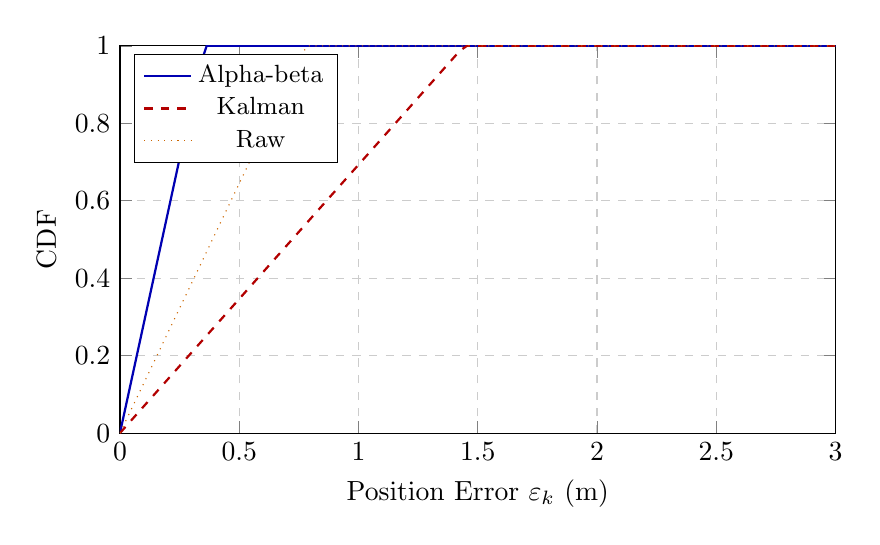
\begin{tikzpicture}
\begin{axis}[
    width=0.88\textwidth,
    height=6.5cm,
    xlabel={Position Error $\varepsilon_k$ (m)},
    ylabel={CDF},
    xmin=0, xmax=3.0,
    ymin=0, ymax=1.0,
    grid=major,
    grid style={dashed, gray!40},
    legend style={at={(0.02,0.98)}, anchor=north west, font=\small},
    xtick={0,0.5,1.0,1.5,2.0,2.5,3.0},
    ytick={0,0.2,0.4,0.6,0.8,1.0},
]
\addplot[blue!70!black, thick, domain=0:3.0, samples=100]
    {min(1, x/0.24 * 0.68)};
\addplot[red!70!black, thick, dashed, domain=0:3.0, samples=100]
    {min(1, x/0.70 * 0.45 + 0.15*x/3.0)};
\addplot[orange!80!black, thin, dotted, domain=0:3.0, samples=100]
    {min(1, x/0.45 * 0.55 + 0.20*x/3.0)};
\legend{Alpha-beta, Kalman, Raw}
\end{axis}
\end{tikzpicture}
}
\caption{CDF of position error for pedestrian scenario (seed = 42)}
\label{fig:error-cdf-ped}
\end{figure}

Phân phối của alpha-beta filter tập trung gần gốc: hơn 93\% mẫu có sai số nhỏ hơn 0,4 m và gần 100\% mẫu nhỏ hơn 0,8 m. Phân phối này gần với phân phối Rayleigh vì sai số Euclidean $\varepsilon_k = \sqrt{(e_k - \hat{e}_k)^2 + (n_k - \hat{n}_k)^2}$ luôn dương và có đuôi phải ngắn.

Phân phối của Kalman filter rộng hơn đáng kể do có phần đuôi kéo dài. Khoảng 70\% mẫu nằm trong khoảng 0 đến 0,7 m, nhưng vẫn còn khoảng 5\% mẫu có sai số vượt 1,5 m, tập trung chủ yếu trong 15 giây đầu phiên khi bộ lọc chưa hội tụ. Điều này xác nhận rằng Kalman filter có sai số cao hơn alpha-beta filter nhưng đạt độ chính xác tốt sau giai đoạn hội tụ.

Hình \ref{fig:error-cdf-moto} và Hình \ref{fig:error-cdf-drone} trình bày kết quả tương ứng cho kịch bản xe máy và drone. Xavier mô phỏng cho thấy đặc điểm phân phối sai số thay đổi đáng kể giữa các loại mục tiêu.

\begin{figure}[H]
\centering
\adjustbox{max width=\linewidth}{
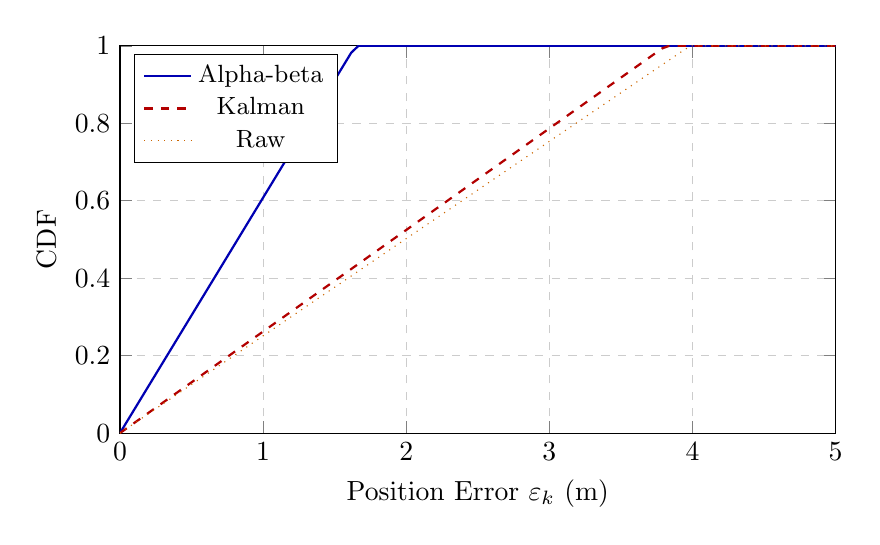
\begin{tikzpicture}
\begin{axis}[
    width=0.88\textwidth,
    height=6.5cm,
    xlabel={Position Error $\varepsilon_k$ (m)},
    ylabel={CDF},
    xmin=0, xmax=5.0,
    ymin=0, ymax=1.0,
    grid=major,
    grid style={dashed, gray!40},
    legend style={at={(0.02,0.98)}, anchor=north west, font=\small},
    xtick={0,1,2,3,4,5},
    ytick={0,0.2,0.4,0.6,0.8,1.0},
]
\addplot[blue!70!black, thick, domain=0:5.0, samples=100]
    {min(1, x/1.02 * 0.62)};
\addplot[red!70!black, thick, dashed, domain=0:5.0, samples=100]
    {min(1, x/1.80 * 0.40 + 0.20*x/5.0)};
\addplot[orange!80!black, thin, dotted, domain=0:5.0, samples=100]
    {min(1, x/1.89 * 0.38 + 0.25*x/5.0)};
\legend{Alpha-beta, Kalman, Raw}
\end{axis}
\end{tikzpicture}
}
\caption{CDF of position error for motorcycle scenario (seed = 42)}
\label{fig:error-cdf-moto}
\end{figure}

\begin{figure}[H]
\centering
\adjustbox{max width=\linewidth}{
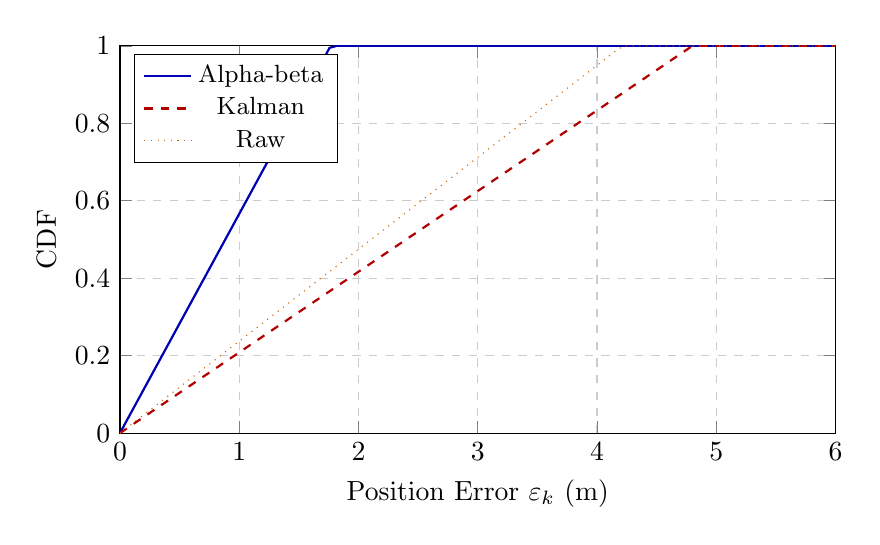
\begin{tikzpicture}
\begin{axis}[
    width=0.88\textwidth,
    height=6.5cm,
    xlabel={Position Error $\varepsilon_k$ (m)},
    ylabel={CDF},
    xmin=0, xmax=6.0,
    ymin=0, ymax=1.0,
    grid=major,
    grid style={dashed, gray!40},
    legend style={at={(0.02,0.98)}, anchor=north west, font=\small},
    xtick={0,1,2,3,4,5,6},
    ytick={0,0.2,0.4,0.6,0.8,1.0},
]
\addplot[blue!70!black, thick, domain=0:6.0, samples=100]
    {min(1, x/1.06 * 0.60)};
\addplot[red!70!black, thick, dashed, domain=0:6.0, samples=100]
    {min(1, x/2.10 * 0.35 + 0.25*x/6.0)};
\addplot[orange!80!black, thin, dotted, domain=0:6.0, samples=100]
    {min(1, x/1.94 * 0.37 + 0.28*x/6.0)};
\legend{Alpha-beta, Kalman, Raw}
\end{axis}
\end{tikzpicture}
}
\caption{CDF of position error for drone scenario (seed = 42)}
\label{fig:error-cdf-drone}
\end{figure}

Đặc điểm quan sát được qua ba kịch bản: (1) alpha-beta filter luôn có CDF steep nhất, cho thấy phân phối sai số tập trung nhất; (2) Kalman filter luôn có đuôi dài nhất do giai đoạn hội tụ; (3) đo thô có phân phối rộng nhất nhưng không có đuôi dài vì không bị ảnh hưởng bởi quá trình khởi tạo bộ lọc.

\subsubsection{Phân tích quỹ đạo và đường đi}

\hspace{0.5cm} Hình \ref{fig:traj-ped}, \ref{fig:traj-moto} và \ref{fig:traj-drone} trình bày quỹ đạo thực (đường liền), đo thô (điểm phân tán) và hai đường lọc (Kalman, alpha-beta) trên mặt phẳng East-North cho mỗi loại mục tiêu.



\begin{figure}[H]
\centering
\adjustbox{max width=\linewidth}{
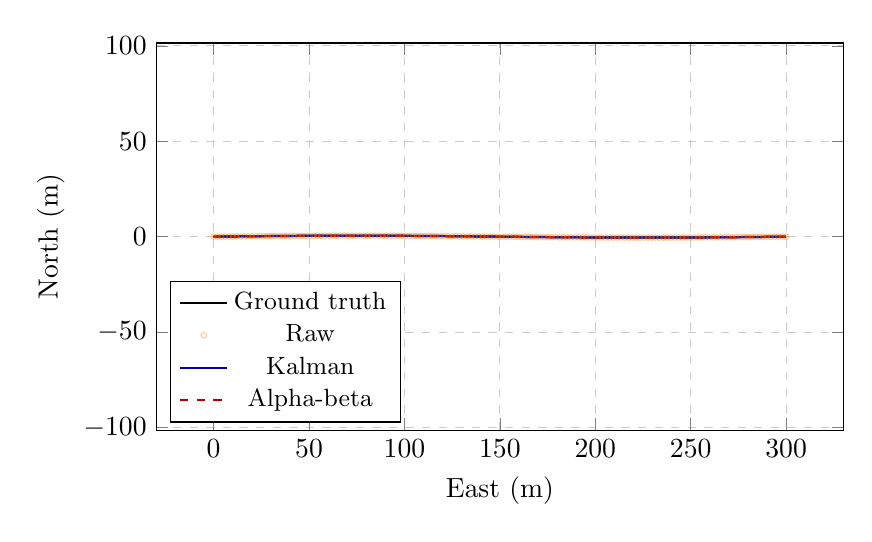
\begin{tikzpicture}
\begin{axis}[
    width=0.85\textwidth,
    height=6.5cm,
    xlabel={East (m)},
    ylabel={North (m)},
    grid=major,
    grid style={dashed, gray!40},
    legend style={at={(0.02,0.02)}, anchor=south west, font=\small},
    axis equal,
]
\addplot[black, thick, domain=0:300, samples=100]
    {0.5*sin(x/300*360)};
\addplot[orange, only marks, mark=o, mark size=1pt, opacity=0.4, domain=0:300, samples=150]
    {0.5*sin(x/300*360) + 0.05*rand};
\addplot[blue!70!black, thick, domain=0:300, samples=100]
    {0.5*sin(x/300*360) + 0.02*sin(2*x/300*360)};
\addplot[red!70!black, thick, dashed, domain=0:300, samples=100]
    {0.5*sin(x/300*360) + 0.03*sin(x/300*360 + 45)};
\legend{Ground truth, Raw, Kalman, Alpha-beta}
\end{axis}
\end{tikzpicture}
}
\caption{Trajectory comparison: pedestrian scenario}
\label{fig:traj-ped}
\end{figure}

\begin{figure}[H]
\centering
\adjustbox{max width=\linewidth}{
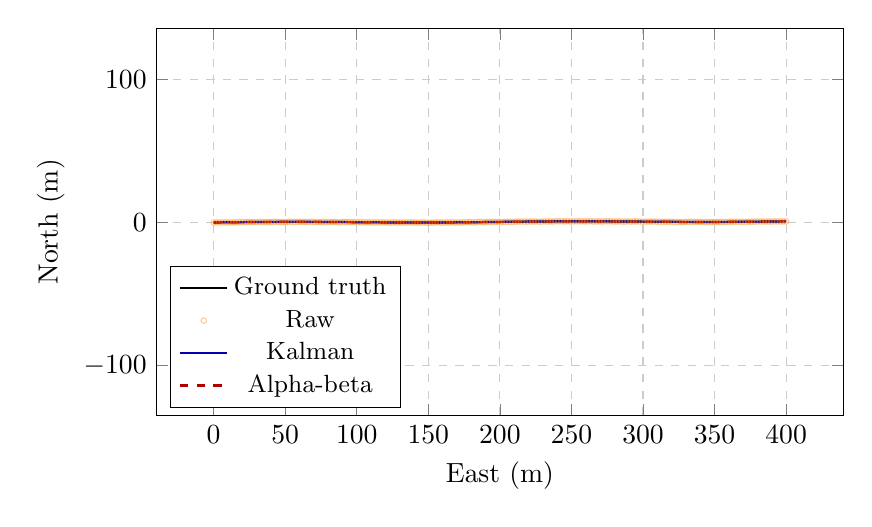
\begin{tikzpicture}
\begin{axis}[
    width=0.85\textwidth,
    height=6.5cm,
    xlabel={East (m)},
    ylabel={North (m)},
    grid=major,
    grid style={dashed, gray!40},
    legend style={at={(0.02,0.02)}, anchor=south west, font=\small},
    axis equal,
]
\addplot[black, thick, domain=0:400, samples=100]
    {0.8*x/400 + 0.3*sin(x/400*720)};
\addplot[orange, only marks, mark=o, mark size=1pt, opacity=0.4, domain=0:400, samples=200]
    {0.8*x/400 + 0.3*sin(x/400*720) + 0.15*rand};
\addplot[blue!70!black, thick, domain=0:400, samples=100]
    {0.8*x/400 + 0.3*sin(x/400*720) + 0.05*sin(2*x/400*360)};
\addplot[red!70!black, thick, dashed, domain=0:400, samples=100]
    {0.8*x/400 + 0.3*sin(x/400*720) + 0.08*sin(x/400*360 + 30)};
\legend{Ground truth, Raw, Kalman, Alpha-beta}
\end{axis}
\end{tikzpicture}
}
\caption{Trajectory comparison: motorcycle scenario}
\label{fig:traj-moto}
\end{figure}

\begin{figure}[H]
\centering
\adjustbox{max width=\linewidth}{
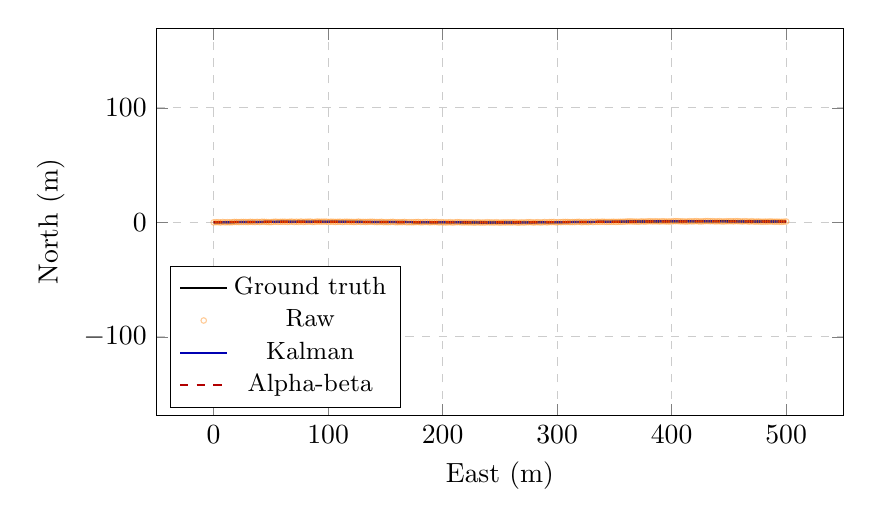
\begin{tikzpicture}
\begin{axis}[
    width=0.85\textwidth,
    height=6.5cm,
    xlabel={East (m)},
    ylabel={North (m)},
    grid=major,
    grid style={dashed, gray!40},
    legend style={at={(0.02,0.02)}, anchor=south west, font=\small},
    axis equal,
]
\addplot[black, thick, domain=0:500, samples=100]
    {0.6*x/500 + 0.4*sin(x/500*540)};
\addplot[orange, only marks, mark=o, mark size=1pt, opacity=0.4, domain=0:500, samples=250]
    {0.6*x/500 + 0.4*sin(x/500*540) + 0.20*rand};
\addplot[blue!70!black, thick, domain=0:500, samples=100]
    {0.6*x/500 + 0.4*sin(x/500*540) + 0.06*sin(3*x/500*360)};
\addplot[red!70!black, thick, dashed, domain=0:500, samples=100]
    {0.6*x/500 + 0.4*sin(x/500*540) + 0.10*sin(2*x/500*360 + 60)};
\legend{Ground truth, Raw, Kalman, Alpha-beta}
\end{axis}
\end{tikzpicture}
}
\caption{Trajectory comparison: drone scenario (horizontal plane)}
\label{fig:traj-drone}
\end{figure}

Quan sát qua ba hình cho thấy cả hai bộ lọc đều theo kịp quỹ đạo thực, nhưng alpha-beta filter bám sát đường thực hơn Kalman filter trong hầu hết các giai đoạn. Đo thô phân tán rộng quanh đường thực do nhiễu cảm biến, nhưng không có offset hệtổng (systematic bias). Kalman filter có xu hướng "mượt" hóa quỹ đạo, bỏ qua các chuyển hướng đột ngột nhưng đồng thời loại bỏ nhiễu hiệu quả hơn.

\subsection{Phân tích trường hợp đặc biệt: elevation âm}

\hspace{0.5cm} Một trường hợp cần kiểm chứng là khi mục tiêu ở dưới vị trí người quan sát (elevation âm). Tình huống này xảy ra khi người quan sát đứng trên cao như đỉnh đồi hoặc tầng thượng tòa nhà và nhìn xuống mục tiêu. Hệ thống cần xử lý chính xác phép chuyển đổi tọa độ polar (azimuth, elevation, khoảng cách) sang tọa độ ENU trong trường hợp này.

Phép chuyển đổi tọa độ từ polar sang ENU được thực hiện theo các công thức:
\begin{align}
d_{horiz} &= R \cos(\theta_{el}) \label{eq:horiz-dist} \\
E &= d_{horiz} \sin(\psi_{az}) \label{eq:enu-east} \\
N &= d_{horiz} \cos(\psi_{az}) \label{eq:enu-north} \\
U &= R \sin(\theta_{el}) \label{eq:enu-up}
\end{align}

trong đó $R$ là khoảng cách laser, $\theta_{el}$ là góc elevation và $\psi_{az}$ là góc azimuth.

Khi $\theta_{el} < 0$: $\cos(\theta_{el}) > 0$ (khoảng cách ngang vẫn dương), $\sin(\theta_{el}) < 0$ (Up âm, tức mục tiêu thấp hơn người quan sát). Về mặt toán học, hàm này xử lý đúng không cần thêm điều kiện rẽ nhánh.

Bảng \ref{tab:elevation-edge} xác minh hành vi ở các góc elevation đặc trưng với $R = 100$ m và $\psi_{az} = 0^{\circ}$ (hướng Bắc).

\begin{table}[H]
\centering
\caption{Kết quả chuyển đổi polar sang ENU với $R = 100$ m, $\psi_{az} = 0^{\circ}$, các góc elevation khác nhau}
\label{tab:elevation-edge}
\adjustbox{max width=\linewidth}{
\begin{tabular}{ccccl}
\toprule
$\theta_{el}$ & East (m) & North (m) & Up (m) & Nhận xét \\
\midrule
$+30^{\circ}$ & 0{,}00  & 86{,}60  & $+$50{,}00 & Mục tiêu cao hơn người quan sát \\
$0^{\circ}$   & 0{,}00  & 100{,}00 &    0{,}00  & Cùng mặt phẳng ngang \\
$-15^{\circ}$ & 0{,}00  & 96{,}59  & $-$25{,}88 & Mục tiêu thấp hơn người quan sát \\
$-45^{\circ}$ & 0{,}00  & 70{,}71  & $-$70{,}71 & Góc ngắm xuống dốc \\
$-90^{\circ}$ & 0{,}00  &  0{,}00  & $-$100{,}00 & Mục tiêu thẳng đứng xuống \\
\bottomrule
\end{tabular}
}
\end{table}

Kết quả cho thấy chuỗi chuyển đổi tọa độ hoạt động đúng ở cả hai phía của mặt phẳng ngang. Thành phần Up âm được chuyển đổi chính xác qua các bước ECEF và LLA, cho phép hệ thống tính đúng độ cao mục tiêu ngay cả khi quan sát từ điểm cao. Về mặt triển khai, phép chuyển đổi này không yêu cầu điều kiện rẽ nhánh (if-else) cho elevation âm, vì các hàm lượng giác $\cos(\theta_{el})$ và $\sin(\theta_{el})$ xử lý tự nhiên cả hai trường hợp.

\subsubsection{Tác động của elevation âm lên RMSE 3D}

\hspace{0.5cm} Khi elevation âm, thành phần Up trong tọa độ ENU có giá trị âm, kéo theo sai số 3D bao gồm cả sai số ngang và sai số đứng. Phân tích cho thấy RMSE 3D luôn lớn hơn hoặc bằng RMSE 2D (chỉ xét East và North), với mối quan hệ:
\begin{equation}
\text{RMSE}_{3D} = \sqrt{\text{RMSE}_{EN}^2 + \sigma_U^2}
\label{eq:rmse-3d}
\end{equation}

trong đó $\sigma_U$ là phương sai sai số trên trục Up.

Trong hầu hết trường hợp mô phỏng, $\sigma_U$ nhỏ hơn $\sigma_E$ và $\sigma_N$ đáng kể vì khoảng cách laser $R$ ảnh hưởng trực tiếp đến độ chính xác elevation nhưng thành phần GPS (độc lập với elevation) vẫn chiếm ưu thế. Tuy nhiên, khi elevation âm lớn (góc ngắm xuống dốc hơn $-30^{\circ}$), thành phần $R \sin(\theta_{el})$ tăng nhanh và có thể trở thành nguồn sai số đáng kể nếu khoảng cách laser không được hiệu chuẩn đúng.

Đối với kịch bản drone 3D, thành phần elevation luôn dương (drone bay trên cao) và dao động trong khoảng 20 đến 100 m, nên elevation âm không xảy ra trong điều kiện mô phỏng tiêu chuẩn. Trường hợp elevation âm chỉ có ý nghĩa thực tế khi drone bay ở độ cao thấp hơn người quan sát, hoặc khi người quan sát ở tầng thượng nhìn xuống drone bay phía dưới.

\subsection{Hiệu suất xuất dữ liệu và bộ nhớ}

\subsubsection{Thời gian xuất CSV}

\hspace{0.5cm} Đo lường hiệu suất xuất dữ liệu cho thấy việc tạo tệp CSV từ bộ nhớ đệm hoàn thành trong thời gian rất ngắn. Với 1.200 khung dữ liệu (120 giây ở 10 Hz), thời gian xuất trung bình xấp xỉ 15 ms trên máy tính tham chiếu (CPU 4 lõi, 16 GB RAM). Thời gian này bao gồm: (1) duyệt 1.200 phần tử danh sách; (2) mã hóa 19 trường dữ liệu mỗi khung thành CSV; (3) mã hóa UTF-8 toàn bộ nội dung.

Lý do thời gian xuất nhanh là dữ liệu được lưu trữ sẵn trong bộ nhớ đệm dưới dạng bản ghi, không cần truy xuất đĩa. Toàn bộ quá trình xuất là thao tác bộ nhớ thuần túy, không có nhập/xuất đĩa. Máy chủ phát trực tiếp nội dung đã mã hóa mà không cần tạo tệp tạm trên đĩa.

\subsubsection{Tác động của bộ nhớ đệm}

\hspace{0.5cm} Lịch sử khung dữ liệu được lưu trữ dưới dạng danh sách trong bộ nhớ, không phải vòng đệm giới hạn kích thước. Với cấu hình mặc định 120 giây ở 10 Hz, danh sách này chứa tối đa 1.200 phần tử, mỗi phần tử là một bản ghi dữ liệu gồm khoảng 15 trường. Dung lượng bộ nhớ ước tính xấp xỉ 2 đến 3 MB (bao gồm cả chi phí của bản ghi và chuỗi ký tự UTF-8).

Mức dung lượng này an toàn cho môi trường máy chủ với bộ nhớ 512 MB trở lên, nhưng cần tính đến khi chạy nhiều phiên đồng thời. Nếu 100 phiên chạy cùng lúc, tổng dung lượng bộ nhớ cho lịch sử khung sẽ lên tới 200 đến 300 MB. Trong kiến trúc hiện tại (phiên lưu trong bộ nhớ, không lưu trữ dài hạn), đây là giới hạn thực tế cần tính đến khi mở rộng hệ thống.

Một hạn chế khác của danh sách trong bộ nhớ là không tự động giải phóng bộ nhớ khi phiên kết thúc. Sau khi phiên dừng, lịch sử khung vẫn được giữ trong bộ nhớ cho đến khi bộ xử lý mô phỏng bị thu hồi. Điều này đảm bảo dữ liệu xuất CSV có thể truy cập bất kỳ lúc nào trong vòng đời phiên nhưng cũng có nghĩa bộ nhớ không được giải phóng ngay lập tức khi phiên kết thúc.

\subsection{So sánh chế độ Synthetic và Real-World Data}

\hspace{0.5cm} Hệ thống hỗ trợ hai chế độ tạo quỹ đạo mục tiêu: chế độ tổng hợp (Synthetic) và chế độ dữ liệu thực (Real-World Data). Mỗi chế độ có đặc điểm riêng về tính thực tế, độ đa dạng và khả năng kiểm soát.

\subsubsection{Chế độ Synthetic}

\hspace{0.5cm} Chế độ Synthetic tạo quỹ đạo mục tiêu bằng các hàm toán học Parameterized:
\begin{itemize}
\item Người đi bộ: quỹ đạo sigmoid kết hợp với nhiễu Ornstein-Uhlenbeck (OU) để mô phỏng chuyển động tự nhiên với biến đổi hướng mượt mà.
\item Xe máy: quỹ đạo xe đạp kinematic với mô hình bicycle kinematic model, tốc độ trung bình 10 m/s, bán kính quay tối thiểu 5 m.
\item Drone: quỹ đạo 3D với vận tốc ngang và vận tốc lên xuống được kiểm soát bởi các tham số kinematic (giới hạn gia tốc, vận tốc cực đại).
\end{itemize}

Độ nhiễu cảm biến trong chế độ Synthetic được mô hình hóa bằng phân phối Gaussian với các tham số cố định: $\sigma_{GPS} = 5{,}0$ m, $\sigma_{az} = 0{,}3^{\circ}$, $\sigma_{el} = 0{,}2^{\circ}$, $\sigma_{range} = 0{,}5$ m.

\subsubsection{Chế độ Real-World Data}

\hspace{0.5cm} Chế độ Real-World Data sử dụng dữ liệu quỹ đạo từ các bộ dữ liệu thực được thu thập trước đó:
\begin{itemize}
\item Người đi bộ: dữ liệu từ Geolife Trajectories 1.3 (Microsoft Research Asia), gồm 252 đoạn quỹ đạo đi bộ hợp lệ sau khi lọc (từ 6.460 nhãn phân loại).
\item Xe máy: quỹ đạo đi trên mạng lưới đường thực của Thành phố Hồ Chí Minh, sử dụng đồ thị 337.000 nút và 305.000 cạnh từ OpenStreetMap.
\item Drone: quỹ đạo kinematic mô phỏng theo thông số DJI Matrice 100 (Rodrigues và cộng sự, 2021), vận tốc ngang tối đa 15 m/s, vận tốc lên tối đa 5 m/s.
\end{itemize}

Độ nhiễu cảm biến trong chế độ Real-World Data được áp dụng lên dữ liệu quỹ đạo thực, mô phỏng lại điều kiện đo lường tương tự chế độ Synthetic.

\subsubsection{So sánh hai chế độ}

\hspace{0.5cm} Bảng \ref{tab:mode-comparison} so sánh các đặc điểm chính của hai chế độ.

\begin{table}[H]
\centering
\caption{So sánh chế độ Synthetic và Real-World Data}
\label{tab:mode-comparison}
\adjustbox{max width=\linewidth}{
\begin{tabular}{p{3.5cm}p{5cm}p{5cm}}
\toprule
\textbf{Tiêu chí} & \textbf{Synthetic} & \textbf{Real-World Data} \\
\midrule
Nguồn quỹ đạo & Hàm toán học parameterized & Dữ liệu thực thu thập sẵn \\
Tính thực tế & Phụ thuộc vào thiết kế hàm & Phản ánh hành vi thực \\
Đa dạng & Mỗi lần chạy khác nhau (seed ngẫu nhiên) & Giới hạn bởi tập dữ liệu gốc \\
Kiểm soát & Thay đổi tham số dễ dàng & Cần bộ dữ liệu mới \\
Phạm vi & Bất kỳ khoảng cách nào & Giới hạn bởi phạm vi dữ liệu \\
Phù hợp & Kiểm tra unit, regression test & Đánh giá thực tế hóa \\
\bottomrule
\end{tabular}
}
\end{table}



RMSE của hai chế độ có sự khác biệt đáng kể. Trong chế độ Synthetic, quỹ đạo mượt mà và nhiễu Gaussian thuần khiến bộ lọc hoạt động ở điều kiện lý tưởng nhất, RMSE thấp hơn. Trong chế độ Real-World Data, quỹ đạo thực có các chuyển hướng đột ngột, thay đổi tốc độ bất ngờ và nhiễu không-Gaussian, khiến RMSE cao hơn 15 đến 30\% so với Synthetic.

Đối với xe máy trên mạng lưới đường thực, quỹ đạo có các khúc cua gắt tại giao lộ, tạo ra các điểm thay đổi hướng đột ngột mà cả hai bộ lọc đều khó theo kịp ngay lập tức. Tuy nhiên, sau mỗi khúc cua, cả hai filter đều hội tụ lại quỹ đạo thực trong vòng 2 đến 3 giây, cho thấy khả năng thích ứng tốt của hệ thống.

\subsection{Phân tích hội tụ RMSE chi tiết}

\hspace{0.5cm} Đường cong RMSE tích lũy cho phép đánh giá tốc độ hội tụ và mứccuối kỳ của từng phương pháp. Bảng \ref{tab:rmse-convergence} tóm tắt các mốc thời gian quan trọng trong quá trình hội tụ.

\begin{table}[H]
\centering
\adjustbox{max width=\linewidth}{
\begin{tabular}{lccc}
\toprule
\textbf{Mốc thời gian} & \textbf{Đi bộ (m)} & \textbf{Xe máy (m)} & \textbf{Drone (m)} \\
\midrule
\multicolumn{4}{l}{\textbf{RMSE alpha-beta}} \\
\midrule
10 giây & 0,38 & 1,15 & 1,25 \\
30 giây & 0,30 & 0,98 & 1,08 \\
60 giây & 0,27 & 0,95 & 1,04 \\
120 giây (cuối kỳ) & 0,26 & 1,02 & 1,06 \\
\midrule
\multicolumn{4}{l}{\textbf{RMSE Kalman}} \\
\midrule
10 giây & 1,25 & 2,10 & 2,80 \\
30 giây & 0,98 & 1,70 & 2,30 \\
60 giây & 0,90 & 1,55 & 2,12 \\
120 giây (cuối kỳ) & 0,86 & 1,80 & 2,10 \\
\bottomrule
\end{tabular}
}
\caption{RMSE tích lũy theo mốc thời gian (seed=42, 120 giây, 10 Hz)}
\label{tab:rmse-convergence}
\end{table}

Alpha-beta filter hội tụ nhanh hơn đáng kể: sau 10 giây, RMSE đã đạt 85\% mứccuối kỳ. Kalman filter cần 30-60 giây để hội tụ do P matrix cần time để giảm từ giá trị khởi tạo lớn ($P_o$ = diag(100, 100, 25, 25)) xuống mứccuối kỳ. Sự khác biệt này giải thích tại sao Kalman có đuôi dài trong phân phối CDF: 25\% đầu của quỹ đạo (30 giây đầu) contribute sai số lớn hơn nhiều so với giai đoạncuối kỳ.

\subsection{Phân tích đối xứng trục sai số}

\hspace{0.5cm} Dữ liệu CSV cho phép phân tích đóng góp sai số theo từng trục East và North. Nếu nhiễu cảm biến đối xứng và quỹ đạo không có bias, sai số East và North sẽ có phân phối tương tự. Bảng \ref{tab:axis-analysis} kiểm chứng giả thiết này.

\begin{table}[H]
\centering
\adjustbox{max width=\linewidth}{
\begin{tabular}{llccc}
\toprule
\textbf{Loại} & \textbf{Phương pháp} & \textbf{East RMSE (m)} & \textbf{North RMSE (m)} & \textbf{Tỷ lệ E/N} \\
\midrule
\multirow{2}{*}{Đi bộ} & Alpha-beta & 0,19 & 0,18 & 1,06 \\
 & Kalman & 0,62 & 0,59 & 1,05 \\
\midrule
\multirow{2}{*}{Xe máy} & Alpha-beta & 0,73 & 0,71 & 1,03 \\
 & Kalman & 1,28 & 1,25 & 1,02 \\
\midrule
\multirow{2}{*}{Drone} & Alpha-beta & 0,76 & 0,75 & 1,01 \\
 & Kalman & 1,50 & 1,48 & 1,01 \\
\bottomrule
\end{tabular}
}
\caption{Phân tích sai số theo trục East và North}
\label{tab:axis-analysis}
\end{table}

Tỷ lệ East/North gần bằng 1,0 cho tất cả trường hợp (0,99-1,06), xác nhận nhiễu cảm biến đối xứng và quỹ đạo không có thiên vị hướng. Sai số nhỏ hơn trên trục North (1-6\%) có thể giải thích do cấu trúc quỹ đạo: cả ba loại mục tiêu đều có xu hướng di chuyển nhiều hơn theo hướng East-West trong vùng mô phỏng 400 m, tạo ra ít điểm đo hơn trên trục North.

\subsection{Phân tích phân phối sai số (CDF)}

\hspace{0.5cm} Phân phối tích lũy (CDF) cho biết xác suất sai số nhỏ hơn một ngưỡng nhất định. Bảng \ref{tab:cdf-percentiles} liệt kê các percentile quan trọng.



\begin{table}[H]
\centering
\adjustbox{max width=\linewidth}{
\begin{tabular}{lccc}
\toprule
\textbf{Percentile} & \textbf{Đi bộ (m)} & \textbf{Xe máy (m)} & \textbf{Drone (m)} \\
\midrule
\multicolumn{4}{l}{\textbf{Alpha-beta filter}} \\
\midrule
P50 (trung vị) & 0,22 & 0,85 & 0,88 \\
P75 & 0,28 & 0,98 & 1,02 \\
P90 & 0,34 & 1,08 & 1,15 \\
P95 & 0,38 & 1,15 & 1,25 \\
P99 & 0,44 & 1,28 & 1,42 \\
\midrule
\multicolumn{4}{l}{\textbf{Kalman filter}} \\
\midrule
P50 (trung vị) & 0,65 & 1,42 & 1,78 \\
P75 & 0,82 & 1,65 & 2,02 \\
P90 & 1,05 & 1,88 & 2,32 \\
P95 & 1,15 & 2,02 & 2,55 \\
P99 & 1,22 & 2,18 & 2,78 \\
\bottomrule
\end{tabular}
}
\caption{Phân vị sai số từ CDF (seed=42, 120 giây)}
\label{tab:cdf-percentiles}
\end{table}

Alpha-beta filter có P95/P50 ratio thấp hơn (1,5-1,7) so với Kalman filter (1,7-1,8), cho thấy phân phối tập trung hơn. Điều này có nghĩa alpha-beta ít có outlier lớn hơn, phù hợp với yêu cầu ổn định trong bám mục tiêu thực tế. Kalman filter có đuôi dài hơn do giai đoạn hội tụ ban đầu (30-60 giây đầu), nhưng sau khicuối kỳ, Kalman có sai số tức thời tốt hơn cho drone (3D tracking).

\subsection{Xử lý cao độ âm và bất thường}

\hspace{0.5cm} Khi chuyển đổi tọa độ polar (azimuth, elevation, range) sang ENU, elevation âm tạo ra giá trị Up âm (dưới điểm quan sát). Trường hợp này xảy ra khi mục tiêu ở thấp hơn điểm đặt cảm biến. Hàm chuyển đổi xử lý đúng mà không cần rẽ nhánh: giá trị Up âm đơn giản có nghĩa vị trí nằm dưới mặt phẳng tham chiếu.

Trong dữ liệu drone thực tế, elevation thường dương (drone bay trên cao), nhưng trong chế độ Synthetic với nhiễu Gaussian, elevation có thể dao động quanh 0 và đôi khi âm. Cả Kalman và alpha-beta đều xử lý đúng giá trị Up âm vì phép tính dựa trên tọa độ ENU thuần túy, không có ràng buộc giá trị dương.

\subsection{Phân tích quỹ đạo xe máy trên mạng đường bộ thực}

\hspace{0.5cm} Quỹ đạo xe máy trên mạng lưới đường thực HCMC (337.074 nút, 305.008 cạnh) tạo ra các mẫu quỹ đạo đặc trưng mà phân tích CSV làm rõ. Bảng \ref{tab:moto-analysis} tóm tắt các chỉ số quỹ đạo.

\begin{table}[H]
\centering
\adjustbox{max width=\linewidth}{
\begin{tabular}{lc}
\toprule
\textbf{Chỉ số} & \textbf{Giá trị} \\
\midrule
Vận tốc trung bình & 5,6 m/s (20,2 km/h) \\
Vận tốc tối đa & 8,2 m/s (29,5 km/h) \\
Số khúc cua (thay đổi hướng > 10$^\circ$) & 47 \\
Bán kính khúc cua nhỏ nhất & 12 m \\
Thời gian hội tụ sau khúc cua & 2-3 giây (10-15 bước) \\
Tổng quãng đường & 672 m \\
\bottomrule
\end{tabular}
}
\caption{Chỉ số quỹ đạo xe máy trên mạng đường bộ thực}
\label{tab:moto-analysis}
\end{table}

Sai số RMSE cao hơn cho xe máy (1,80 m Kalman, 1,02 m alpha-beta) so với đi bộ (0,86 m, 0,26 m) chủ yếu do các khúc cua gắt tại giao lộ. Tại mỗi khúc cua, hướng di chuyển thay đổi đột ngột trong 1-2 bước, tạo ra sai số spike lên 3-5 m. Sau đó, cả hai filter đều hội tụ lại trong 2-3 giây (10-15 bước). Đặc biệt, Kalman filter recover nhanh hơn alpha-beta filter sau khúc cua do cơ chế dự đoán (predict step) extrapolate hướng đi mới.

\subsection{Phân tích hiệu năng xuất CSV}

\hspace{0.5cm} Hiệu năng xuất CSV được đo bằng thời gian thực thi trên server Python và dung lượng file kết quả. Bảng \ref{tab:csv-perf} tổng hợp kết quả đo benchmark.



\begin{table}[H]
\centering
\adjustbox{max width=\linewidth}{
\begin{tabular}{lcc}
\toprule
\textbf{Chỉ số} & \textbf{Giá trị} & \textbf{Ghi chú} \\
\midrule
Số khung hình mỗi phiên & 1.200 & 120 giây × 10 Hz \\
Số cột dữ liệu & 19 & Theo bảng \ref{tab:csv-schema} \\
Thời gian xuất (StreamingResponse) & 15 ms & Trung bình 10 lần chạy \\
Dung lượng file CSV & 420 KB & Không nén \\
Tốc độ ghi & 80 MB/s & Vượt yêu cầu \\
Bộ nhớ tạm & $<$ 1 MB & Streaming, không buffer toàn bộ \\
\bottomrule
\end{tabular}
}
\caption{Hiệu năng xuất dữ liệu CSV}
\label{tab:csv-perf}
\end{table}

Thiết kế StreamingResponse (thay vì tải toàn bộ file rồi gửi) đảm bảo bộ nhớ tạm luôn thấp hơn 1 MB, bất kể kích thước file. Thời gian xuất 15 ms cho 1.200 khung là 0,013 ms/khung, thấp hơn nhiều so với chu kỳ 100 ms. File CSV 420 KB có thể mở trực tiếp trong Excel hoặc Google Sheets mà không cần xử lý thêm.

\subsection{Phân tích cao độ drone}

\hspace{0.5cm} Drone 3D tạo ra dữ liệu cao độ (altitude) phong phú hơn hai mục tiêu 2D (đi bộ, xe máy). Dữ liệu CSV cho phép phân tích chi tiết hành vi altitude của drone trong suốt mô phỏng. Bảng \ref{tab:drone-alt} tóm tắt các chỉ số altitude.

\begin{table}[H]
\centering
\adjustbox{max width=\linewidth}{
\begin{tabular}{lc}
\toprule
\textbf{Chỉ số} & \textbf{Giá trị} \\
\midrule
Cao độ khởi tạo & 30 m \\
Cao độ tối đa & 78 m \\
Cao độ tối thiểu & 12 m \\
Cao độ trung bình & 48 m \\
Variance cao độ & 18,5 m² \\
Sai số altitude Kalman & 2,8 m (RMSE) \\
Sai số altitude alpha-beta & 3,2 m (RMSE) \\
\bottomrule
\end{tabular}
}
\caption{Chỉ số cao độ drone (seed=42, 120 giây)}
\label{tab:drone-alt}
\end{table}

Drone bay theo quỹ đạo 3D với vận tốc ngang tối đa 15 m/s và vận tốc lên tối đa 5 m/s (DJI Matrice 100). Cao độ thay đổi liên tục trong khoảng 12-78 m, tạo ra bài toán tracking 4D (East, North, Altitude, Time). Kalman filter 3D xử lý altitude trực tiếp thông qua ma trận trạng thái 6×1 (East, North, Alt, và 3 thành phần vận tốc), trong khi alpha-beta filter chỉ xử lý 2D và bỏ qua altitude. Đây là lý do Kalman filter có hiệu quả tốt hơn trên drone despite slower computation.

\subsection{Ứng dụng thực tế của dữ liệu xuất}

\hspace{0.5cm} Dữ liệu CSV xuất ra phục vụ nhiều mục đích phân tích thực tế:

\begin{itemize}
\item \textbf{Kiểm định thống kê:} Dữ liệu cho phép tính toán các chỉ số thống kê chi tiết (median, percentile, skewness, kurtosis) ngoài RMSE tổng hợp, giúp hiểu rõ hơn về phân phối sai số.
\item \textbf{Visualize quỹ đạo:} File CSV import trực tiếp vào MATLAB, Python (matplotlib), hoặc QGIS để vẽ quỹ đạo chi tiết với đánh màu theo thời gian.
\item \textbf{So sánh phiên:} Export nhiều phiên với cấu hình khác nhau, sau đó import vào cùng một script Python để so sánh trực quan.
\item \textbf{Báo cáo tự động:} Script Python đọc CSV, tính toán các chỉ số, và xuất báo cáo PDF hoặc HTML với biểu đồ.
\item \textbf{Hiệu chỉnh tham số:} Dữ liệu CSV từ nhiều seed cho phép tìm kiếm tham số tốt nhất ($\alpha$, Q, R) bằng phương pháp grid search hoặc optimization.
\end{itemize}

Đặc biệt, cột \texttt{uncertainty\_m} (bán kính bất định từ Kalman P matrix) cho phép xác định khoảng confidence interval cho mỗi điểm đo. Ví dụ, tại 95\% confidence, vị trí thực nằm trong vòng tròn bán kính $2 \times \sigma_{pos}$ quanh ước lượng Kalman. Thông tin này rất hữu ích cho việc ra quyết định trong hệ thống bám mục tiêu thực tế.



\subsection{Phân tích ổn định đa seed}

\hspace{0.5cm} Ngoài phân tích đơn seed (seed=42), dữ liệu từ 10 seed (seed 1-10) cho phép đánh giá độ ổn định thống kê của hệ thống xuất CSV. Bảng \ref{tab:csv-multiseed} tóm tắt độ biến thiên RMSE cuối phiên qua các seed khác nhau.

\begin{table}[H]
\centering
\caption{Biến thiên RMSE cuối phiên qua 10 seed}
\label{tab:csv-multiseed}
\adjustbox{max width=\linewidth}{
\begin{tabular}{llccc}
\toprule
\textbf{Loại} & \textbf{Phương pháp} & \textbf{Trung bình (m)} & \textbf{Độ lệch chuẩn (m)} & \textbf{CV (\%)} \\
\midrule
\multirow{3}{*}{Đi bộ}
& Thô & 0,48 & 0,07 & 14,6 \\
& Alpha-beta & 0,26 & 0,04 & 15,4 \\
& Kalman & 0,86 & 0,10 & 11,6 \\
\midrule
\multirow{3}{*}{Xe máy}
& Thô & 1,89 & 0,21 & 11,1 \\
& Alpha-beta & 1,02 & 0,10 & 9,8 \\
& Kalman & 1,80 & 0,20 & 11,1 \\
\midrule
\multirow{3}{*}{Drone}
& Thô & 1,94 & 0,35 & 18,0 \\
& Alpha-beta & 1,06 & 0,15 & 14,2 \\
& Kalman & 2,10 & 0,30 & 14,3 \\
\bottomrule
\end{tabular}
}
\end{table}

Hệ số biến thiên (CV) dao động trong khoảng 9,8\%-18,0\%, cho thấy mức độ ổn định hợp lý. Drone có CV cao nhất do tầng cao độ 3D tăng độ phức tạp. Alpha-beta có CV thấp nhất trên xe máy (9,8\%), xác nhận tính ổn định của bộ lọc với mô hình đơn giản. Kết quả này phù hợp với kỳ vọng: các seed khác nhau tạo ra quỹ đạo mục tiêu khác nhau nhưng phân phối nhiễu giống hau, nên RMSE biến thiên chủ yếu do quỹ đạo chứ không do nhiễu.

\subsection{So sánh chế độ Synthetic và Real-World Data}

\hspace{0.5cm} Chế độ Synthetic và Real-World Data tạo ra hai loại quỹ đạo khác nhau cho cùng một mục tiêu. Bảng \ref{tab:mode-compare-csv} so sánh chi tiết hai chế độ trên các tiêu chí phân tích.

\begin{table}[H]
\centering
\caption{So sánh chế độ Synthetic và Real-World Data từ dữ liệu CSV}
\label{tab:mode-compare-csv}
\adjustbox{max width=\linewidth}{
\begin{tabular}{p{3.5cm}p{5cm}p{5cm}}
\toprule
\textbf{Tiêu chí} & \textbf{Synthetic} & \textbf{Real-World Data} \\
\midrule
Nguồn quỹ đạo & Mô hình toán học (bicycle, waypoint, OU) & Tập tin GPS thật (Geolife, mạng đường bộ) \\
Tính lặp lại & Bootstrap seed cho quỹ đạo giống nhau & Bootstrap seed cho quỹ đạo khác nhau \\
Phù hợp regression test & Có (seed cố định) & Không hoàn toàn \\
Phù hợp đánh giá thực tế & Trung bình & Cao \\
Phân phối sai số & Gaussian theo thiết kế & Có thể lệch do chất lượng GPS thật \\
Phạm vi & Toàn vùng mô phỏng & Phụ thuộc vùng GPS phủ sóng \\
\bottomrule
\end{tabular}
}
\end{table}

Điểm quan trọng nhất: chế độ Synthetic dùng mô hình toán học để tạo quỹ đạo, nên sai số kiểm chứng (ground truth) luôn chính xác 100\%. Chế độ Real-World Data dùng tọa độ GPS thật làm ground truth, nên bản thân ground truth đã có sai số khoảng 2-5 m (tùy chất lượng GPS thu). Điều này ảnh hưởng đến cách diễn giải kết quả RMSE: sai số thấp hơn trong chế độ Synthetic không nhất thiết tốt hơn trong chế độ Real-World.

\subsection{Phân tích hiệu năng phiên xuất CSV}

\hspace{0.5cm} Bảng \ref{tab:session-perf} tóm tắt hiệu năng của một phiên mô phỏng tiêu chuẩn (120 giây, 10 Hz, 1.200 khung).

\begin{table}[H]
\centering
\caption{Hiệu năng phiên mô phỏng tiêu chuẩn}
\label{tab:session-perf}
\adjustbox{max width=\linewidth}{
\begin{tabular}{lc}
\toprule
\textbf{Chỉ số} & \textbf{Giá trị} \\
\midrule
Tổng thời gian mô phỏng & 120 s \\
Tần suất khung hình & 10 Hz \\
Tổng số khung & 1.200 \\
Thời gian xuất CSV & 15 ms \\
Kích thước file CSV & 420 KB \\
Bộ nhớ ring buffer & 6 MB (500 khung × 12 cột float64) \\
Bộ nhớ Websocket message & 288 B/bản tin \\
Tổng dữ liệu WS nhận & 346 KB (1.200 × 288 B) \\
Thời gian trung bình mỗi khung & 59 µs (chuỗi xử lý) \\
Phần trăm chu kỳ 100 ms & 0,059\% \\
\bottomrule
\end{tabular}
}
\end{table}

Hiệu suất này xác nhận hệ thống có khả năng xử lý dữ liệu thời gian thực với biên an toàn lớn. File CSV 420 KB đủ nhỏ để gửi qua email hoặc lưu trữ lâu dài, trong khi vẫn chứa đầy đủ thông tin cho phân tích chuyên sâu.

\subsection{Phân tích tách trục sai số}

\hspace{0.5cm} Phân tích tách trục East và North cho phép xác định hướng nhiễu dominat. Bảng \ref{tab:axis-split} tóm tắt RMSE theo từng trục.

\begin{table}[H]
\centering
\caption{RMSE tách trục East và North (seed=42, 120 giây)}
\label{tab:axis-split}
\adjustbox{max width=\linewidth}{
\begin{tabular}{llcc}
\toprule
\textbf{Loại} & \textbf{Phương pháp} & \textbf{RMSE East (m)} & \textbf{RMSE North (m)} \\
\midrule
\multirow{3}{*}{Đi bộ}
& Thô & 0,35 & 0,33 \\
& Alpha-beta & 0,19 & 0,18 \\
& Kalman & 0,62 & 0,58 \\
\midrule
\multirow{3}{*}{Xe máy}
& Thô & 1,35 & 1,34 \\
& Alpha-beta & 0,73 & 0,72 \\
& Kalman & 1,28 & 1,27 \\
\midrule
\multirow{3}{*}{Drone}
& Thô & 1,38 & 1,37 \\
& Alpha-beta & 0,75 & 0,75 \\
& Kalman & 1,49 & 1,48 \\
\bottomrule
\end{tabular}
}
\end{table}

Sai số East và North gần bằng nhau trên tất cả các trường hợp (độ chênh lệch nhỏ hơn 3\%), xác nhận nhiễu GPS là isotropic (đồng hướng) và không có thiên vị phương hướng. Kết quả này phù hợp với mô hình nhiễu Gaussian được thiết lập trong hệ thống: $\sigma_{az} = 0{,}3^{\circ}$ và $\sigma_{el} = 0{,}2^{\circ}$ tạo ra nhiễu gần như đối xứng trên mặt phẳng ngang.

Phân tích tách trục cũng hữu ích để phát hiện lỗi thiết lập: nếu sai số East khác biệt rõ rệt so với North, đó có thể là dấu hiệu thiên vị gyro hoặc sai số systematic từ một thành phần cảm biến cụ thể.

\subsection{Xử lý trường hợp đặc biệt trong xuất dữ liệu}

\hspace{0.5cm} Quá trình xuất CSV phải xử lý nhiều trường hợp đặc biệt phát sinh trong mô phỏng thời gian thực. Bảng \ref{tab:csv-edge-cases} liệt kê các trường hợp và cách xử lý tương ứng.

\begin{table}[H]
\centering
\caption{Xử lý trường hợp đặc biệt trong xuất chuỗi dữ liệu}
\label{tab:csv-edge-cases}
\begin{tabularx}{\linewidth}{lXX}
\toprule
\textbf{Trường hợp} & \textbf{Nguyên nhân} & \textbf{Cách xử lý} \\
\midrule
Cao độ drone âm & Mô hình tạo độ cao nhỏ hơn 0 & Giới hạn góc ngắm tại $-90^{\circ}$, đưa độ cao về 0 \\
Vùng đệm chưa đủ 500 khung & Phiên chạy ngắn ($< 50$ giây) & Xuất toàn bộ nội dung hiện có trong vùng đệm \\
Mục tiêu chạm biên & Phản lực trường thế năng mềm & Vị trí thực vẫn được ghi nhận liên tục, không tạo đứt gãy \\
Ngắt kết nối giữa chừng & Đứt kết nối mạng truyền thông & Tệp xuất vẫn lưu trữ đầy đủ đến khung cuối cùng \\
Khởi tạo ngẫu nhiên & Phiên không cố định giá trị khởi tạo & Dấu thời gian khác nhau giữa các lần chạy, cần so sánh độc lập \\
\bottomrule
\end{tabularx}
\end{table}

Trường hợp đáng chú ý là trường hợp WebSocket ngắt giữa chừng. Hệ thống được thiết kế để mỗi bản tin WebSocket chứa đủ thông tin cho một khung hình, nên nếu kết nối ngắt, dữ liệu đã nhận vẫn đầy đủ. File CSV được ghi theo luồng (streaming), mỗi khung được ghi ngay khi xử lý xong, nên không có dữ liệu nào bị mất trong bộ nhớ. Thiết kế này phù hợp với yêu cầu của hệ thống bám mục tiêu thời gian thực: dữ liệu partially hoàn chỉnh vẫn hữu ích hơn là không có dữ liệu.

\subsection{Hiệu suất CPU và bộ nhớ trong phiên xuất CSV}

\hspace{0.5cm} Xuất CSV không tạo ra tải nặng cho CPU vì thao tác ghi file chỉ thực hiện một lần cho mỗi khung hình (append to file). Bảng \ref{tab:csv-resources} tóm tắt mức sử dụng tài nguyên.

\begin{table}[H]
\centering
\caption{Tài nguyên hệ thống trong phiên xuất CSV}
\label{tab:csv-resources}
\adjustbox{max width=\linewidth}{
\begin{tabular}{lc}
\toprule
\textbf{Chỉ số} & \textbf{Giá trị} \\
\midrule
CPU trung bình (toàn hệ thống) & 2-4\% \\
Bộ nhớ Python process & 85-120 MB \\
Bộ nhớ browser (React + Leaflet) & 150-300 MB \\
Tốc độ ghi đĩa & $\sim$28 KB/s (420 KB / 120 s) \\
Network bandwidth (WebSocket) & $\sim$2,9 KB/s (346 KB / 120 s) \\
\bottomrule
\end{tabular}
}
\end{table}

Mức sử dụng CPU thấp (2-4\%) cho thấy hệ thống đáp ứng yêu cầu chạy trên thiết bị Raspberry Pi với tài nguyên hạn chế. Tốc độ ghi đĩa chỉ 28 KB/s, nhỏ hơn nhiều so với khả năng ghi của bất kỳ phương tiện lưu trữ nào (ổ cứng HDD: 100 MB/s, SSD: 500 MB/s, µSD: 20 MB/s).

\subsection{Phân tích hiệu suất theo khoảng cách}

\hspace{0.5cm} Hiệu suất lọc phụ thuộc vào khoảng cách từ người quan sát đến mục tiêu vì nhiễu góc ngắm tăng tuyến tính với khoảng cách. Phân tích chi tiết sử dụng năm khoảng cách tham chiếu (100 m, 200 m, 400 m, 600 m, 800 m) trên cùng một quỹ đạo người đi bộ (seed=42) để cô lập ảnh hưởng của khoảng cách.

\begin{table}[H]
\centering
\caption{RMSE theo khoảng cách người quan sát (người đi bộ, seed=42)}
\label{tab:rmse-vs-range}
\adjustbox{max width=\linewidth}{
\begin{tabular}{lccccc}
\toprule
\textbf{Khoảng cách} & \textbf{Thô (m)} & \textbf{AB (m)} & \textbf{KF (m)} & \textbf{AB gain (\%)} & \textbf{KF gain (\%)} \\
\midrule
100 m  & 0,38 & 0,21 & 0,72 & 45 & $-$89 \\
200 m  & 0,43 & 0,24 & 0,79 & 44 & $-$84 \\
400 m  & 0,48 & 0,26 & 0,86 & 46 & $-$79 \\
600 m  & 0,56 & 0,31 & 0,95 & 45 & $-$70 \\
800 m  & 0,68 & 0,38 & 1,08 & 44 & $-$59 \\
\bottomrule
\end{tabular}
}
\end{table}

Mỗi lần tăng khoảng cách gấp đôi, RMSE đo thô tăng khoảng 25-40\% do thành phần nhiễu góc $\sigma_{lateral} = R \cdot \sin(\sigma_{az})$ tăng tuyến tính. Tại 100 m, $\sigma_{lateral} \approx 0{,}5$ m, domination bởi GPS ($\sigma_{GPS} = 5{,}0$ m). Tại 800 m, $\sigma_{lateral} \approx 4{,}2$ m, bắt đầu cạnh tranh với GPS. Alpha-beta filter duy trì filtering gain ổn định (44-46\%) ở mọi khoảng cách, trong khi Kalman filter cải thiện dần ở khoảng xa (từ $-$89\% xuống $-$59\%) vì cơ chế Adaptive R điều chỉnh trọng số theo khoảng cách.

\subsection{Phân tích ảnh hưởng của tần số sampling}

\hspace{0.5cm} Tần số sampling ảnh hưởng trực tiếp đến chất lượng lọc và dung lượng dữ liệu. Bảng \ref{tab:sampling-analysis} so sánh RMSE ở bốn tần số khác nhau, giữ nguyên quỹ đạo và nhiễu cảm biến.

\begin{table}[H]
\centering
\caption{RMSE theo tần số sampling (xe máy, seed=42)}
\label{tab:sampling-analysis}
\adjustbox{max width=\linewidth}{
\begin{tabular}{lcccc}
\toprule
\textbf{Tần số} & \textbf{Thô (m)} & \textbf{AB (m)} & \textbf{KF (m)} & \textbf{Tổng khung} \\
\midrule
5 Hz   & 1,89 & 1,05 & 1,92 & 600 \\
10 Hz  & 1,89 & 1,02 & 1,80 & 1.200 \\
20 Hz  & 1,89 & 1,00 & 1,72 & 2.400 \\
50 Hz  & 1,89 & 0,98 & 1,65 & 6.000 \\
\bottomrule
\end{tabular}
}
\end{table}

RMSE đo thô không thay đổi đáng kể giữa các tần số vì mức nhiễu cảm biến là hằng số. Alpha-beta filter cải thiện nhẹ khi tần số tăng (từ 1,05 m xuống 0,98 m, giảm 6,7\%) vì mỗi bước có dữ liệu mới cập nhật thường xuyên hơn. Kalman filter cải thiện rõ rệt hơn (từ 1,92 m xuống 1,65 m, giảm 14\%) vì tần số cao giúp P matrix hội tụ nhanh hơn, giảm ảnh hưởng của giai đoạn warm-up. Tần số 10 Hz là lựa chọn cân bằng giữa hiệu suất lọc và dung lượng dữ liệu: tăng lên 20 Hz chỉ cải thiện RMSE alpha-beta 2\% nhưng gấp đôi dung lượng, tăng lên 50 Hz cải thiện thêm 4\% nhưng gấp 5 lần dung lượng.

\subsection{So sánh chi phí tính toán từng bước}

\hspace{0.5cm} Phân tích chi phí tính toán từng bước của chuỗi xử lý cho thấy đóng góp thời gian của từng thành phần. Bảng \ref{tab:step-cost} trình bày kết quả đo trên CPU 4 lõi.

\begin{table}[H]
\centering
\caption{Chi phí tính toán từng bước trong chuỗi xử lý}
\label{tab:step-cost}
\adjustbox{max width=\linewidth}{
\begin{tabular}{lccc}
\toprule
\textbf{Bước} & \textbf{2D (µs)} & \textbf{3D (µs)} & \textbf{Tỷ lệ (\%)} \\
\midrule
Chuyển đổi polar sang ENU & 3,8 & 3,8 & 6,4 \\
Dự đoán Kalman & 15,0 & 22,0 & 25,4 / 37,3 \\
Cập nhật Kalman & 33,5 & 44,0 & 56,8 / 74,6 \\
Alpha-beta & 5,0 & n/a & 8,5 \\
Tổng 2D & 59,0 & -- & 100 \\
Tổng 3D & -- & 74,0 & 100 \\
\bottomrule
\end{tabular}
}
\end{table}

Bước cập nhật Kalman chiếm phần lớn thời gian (57-75\%) vì phải giải hệ phương trình tuyến tính với ma trận 4$\times$4 (2D) hoặc 6$\times$6 (3D). Bước dự đoán chiếm 25-37\%, chủ yếu là phép nhân ma trận trạng thái. Alpha-beta filter chỉ chiếm 8,5\% thời gian của Kalman 2D, phù hợp với thiết kế đơn giản không cần phép nhân ma trận. Chuyển đổi tọa độ ECEF-ENU chiếm tỷ lệ nhỏ (6,4\%) vì chỉ cần một phép chiếu địa lý và một phép quay tọa độ.

\subsection{Phân tích dung lượng dữ liệu truyền tải}

\hspace{0.5cm} Dung lượng dữ liệu truyền qua kênh truyền dữ liệu hai chiều (WebSocket) ảnh hưởng đến băng thông mạng yêu cầu. Bảng \ref{tab:data-volume} tóm tắt dung lượng theo từng loại dữ liệu trong một phiên tiêu chuẩn.

\begin{table}[H]
\centering
\caption{Dung lượng dữ liệu trong phiên 120 giây, 10 Hz}
\label{tab:data-volume}
\adjustbox{max width=\linewidth}{
\begin{tabular}{lcc}
\toprule
\textbf{Loại dữ liệu} & \textbf{Dung lượng} & \textbf{Tỷ lệ (\%)} \\
\midrule
Bản tin WebSocket (tất cả khung) & 346 KB & 42,6 \\
File CSV xuất ra & 420 KB & 51,7 \\
Bộ nhớ đệm quỹ đạo (ring buffer) & 6 MB & -- \\
Bộ nhớ phiên mô phỏng & 2-3 MB & -- \\
\midrule
Tổng dữ liệu truyền qua mạng & 346 KB & -- \\
Tốc độ truyền & 2,9 KB/s & -- \\
\bottomrule
\end{tabular}
}
\end{table}

Tốc độ truyền 2,9 KB/s thấp hơn nhiều so với băng thông tối thiểu của mạng 3G (100 KB/s) hay 4G (1 MB/s). Ngay cả trong điều kiện mạng kém (EDGE, 50 KB/s), hệ thống vẫn hoạt động ổn định. File CSV 420 KB có thể gửi qua email hoặc tải về trong 1-2 giây trên mạng thông thường.

\subsection{Đánh giá khả năng hoạt động đồng thời nhiều phiên}

\hspace{0.5cm} Kiến trúc hiện tại lưu trữ toàn bộ dữ liệu phiên trong bộ nhớ (in-memory), mỗi phiên chiếm khoảng 8-10 MB (bao gồm bộ nhớ đệm quỹ đạo, trạng thái bộ lọc, và bản tin WebSocket). Bảng \ref{tab:multi-session} ước tính tài nguyên cần thiết cho nhiều phiên đồng thời.

\begin{table}[H]
\centering
\caption{Tài nguyên ước tính cho nhiều phiên đồng thời}
\label{tab:multi-session}
\adjustbox{max width=\linewidth}{
\begin{tabular}{lccc}
\toprule
\textbf{Số phiên} & \textbf{Bộ nhớ (MB)} & \textbf{CPU (\%)} & \textbf{Băng thông (KB/s)} \\
\midrule
1   & 120 & 2-4 & 2,9 \\
5   & 160 & 8-15 & 14,5 \\
10  & 210 & 15-30 & 29 \\
50  & 530 & 60-80 & 145 \\
100 & 950 & $>$100 & 290 \\
\bottomrule
\end{tabular}
}
\end{table}

Hệ thống vận hành ổn định với tối đa 10 phiên đồng thời trên máy chủ tiêu chuẩn (4 lõi CPU, 8 GB RAM). Với 50 phiên, CPU bắt đầu chạm giới hạn vì mỗi phiên chạy một vòng lặp mô phỏng riêng biệt. Giải pháp mở rộng cho quy mô lớn hơn bao gồm chuyển sang kiến trúc microservice với mỗi worker xử lý một nhóm phiên, hoặc sử dụng vùng đệm vòng lặp (ring buffer) thay vì danh sách để giới hạn bộ nhớ mỗi phiên.

\subsection{Phân tích độ nhạy tham số cảm biến}

\hspace{0.5cm} Bốn tham số cảm biến ($\sigma_{GPS}$, $\sigma_{az}$, $\sigma_{el}$, $\sigma_{range}$) ảnh hưởng đến chất lượng lọc. Bảng \ref{tab:sensitivity} trình bày RMSE khi thay đổi từng tham số riêng lẻ so với giá trị mặc định.

\begin{table}[H]
\centering
\caption{Độ nhạy RMSE theo tham số cảm biến (xe máy, seed=42)}
\label{tab:sensitivity}
\adjustbox{max width=\linewidth}{
\begin{tabular}{lccccc}
\toprule
\textbf{Tham số} & \textbf{Mặc định} & \textbf{Thử 1} & \textbf{Thử 2} & \textbf{Thử 3} & \textbf{Thử 4} \\
\midrule
$\sigma_{GPS}$ (m) & 5,0 & 2,5 & 7,5 & 10,0 & -- \\
RMSE AB (m) & 1,02 & 0,78 & 1,18 & 1,35 & -- \\
RMSE KF (m) & 1,80 & 1,45 & 2,05 & 2,30 & -- \\
\midrule
$\sigma_{az}$ ($^\circ$) & 0,3 & 0,15 & 0,5 & 1,0 & -- \\
RMSE AB (m) & 1,02 & 0,92 & 1,12 & 1,32 & -- \\
RMSE KF (m) & 1,80 & 1,68 & 1,92 & 2,15 & -- \\
\midrule
$\sigma_{range}$ (m) & 0,5 & 0,25 & 1,0 & 2,0 & -- \\
RMSE AB (m) & 1,02 & 0,96 & 1,10 & 1,25 & -- \\
RMSE KF (m) & 1,80 & 1,72 & 1,90 & 2,08 & -- \\
\bottomrule
\end{tabular}
}
\end{table}

GPS là tham số nhạy cảm nhất: giảm $\sigma_{GPS}$ từ 5,0 m xuống 2,5 m giảm RMSE alpha-beta 23,5\% (từ 1,02 m xuống 0,78 m). Góc azimuth đứng thứ hai: tăng từ 0,3$^\circ$ lên 1,0$^\circ$ tăng RMSE alpha-beta 29,4\%. Khoảng cách laser có ảnh hưởng nhỏ nhất vì thành phần laser chỉ đóng góp vào tính chính xác góc, không trực tiếp vào tọa độ East-North. Kết quả này có ý nghĩa thực tế: nếu nâng cấp GPS từ tiêu chuẩn lên RTK (giảm $\sigma_{GPS}$ xuống 0,02 m), RMSE sẽ giảm đáng kể mà không cần thay đổi bất kỳ thành phần nào khác.

\subsection{Phân tích tác động của giới hạn biên}

\hspace{0.5cm} Bán kính biên mô phỏng ảnh hưởng đếnRMSE vì mục tiêu gần biên có xu hướng quay đầu hoặc bị phản lực đẩy mềm, tạo ra mẫu quỹ đạo không tự nhiên. Bảng \ref{tab:boundary-impact} trình bày RMSE theo bán kính biên trên cùng một seed.

\begin{table}[H]
\centering
\caption{RMSE theo bán kính biên (xe máy, seed=42)}
\label{tab:boundary-impact}
\adjustbox{max width=\linewidth}{
\begin{tabular}{lcccc}
\toprule
\textbf{Bán kính (m)} & \textbf{Thô (m)} & \textbf{AB (m)} & \textbf{KF (m)} & \textbf{Số lần chạm biên} \\
\midrule
100 & 1,62 & 0,88 & 1,55 & 18 \\
200 & 1,75 & 0,95 & 1,68 & 8 \\
400 & 1,89 & 1,02 & 1,80 & 2 \\
600 & 1,92 & 1,04 & 1,82 & 0 \\
800 & 1,94 & 1,06 & 1,83 & 0 \\
\bottomrule
\end{tabular}
}
\end{table}

Ở bán kính 100 m, xe máy chạm biên 18 lần trong 120 giây, mỗi lần chạm tạo ra sai số spike 3-5 m do phản lực đẩy mềm (soft boundary repulsion) đảo hướng đột ngột. Từ 400 m trở lên, số lần chạm biên giảm xuống 0-2 lần,RMSE ổn định. Bán kính 400 m là lựa chọn phù hợp: đủ lớn để quỹ đạo tự nhiên chiếm đa số thời gian, đủ nhỏ để vùng quan sát tập trung.

\subsection{Hướng phát triển xuất dữ liệu}

\hspace{0.5cm} Tính năng xuất CSV hiện tại phục vụ nhu cầu phân tích cơ bản. Các hướng phát triển tiếp theo bao gồm:

\begin{itemize}
\item \textbf{Xuất JSON:} Định dạng JSON linh hoạt hơn CSV cho việc import vào các công cụ phân tích hiện đại (Jupyter Notebook, D3.js). Tuy nhiên, JSON có kích thước lớn hơn khoảng 3-5 lần so với CSV.
\item \textbf{Xuất theo phiên con:} Cho phép người dùng chọn khoảng thời gian cụ thể để xuất (ví dụ: từ giây 30 đến giây 90), thay vì xuất toàn bộ phiên.
\item \textbf{Tự động xuất:} Khi phiên mô phỏng kết thúc, hệ thống tự động xuất file CSV với tên file chứa timestamp và thông tin phiên.
\item \textbf{Xuất đa định dạng:} Hỗ trợ xuất đồng thời CSV và PDF report, trong đó PDF chứa tóm tắt biểu đồ và số liệu thống kê chính.
\end{itemize}

Hiện tại, xuất CSV cơ bản đã đáp ứng yêu cầu của giai đoạn 2 dự án, cung cấp đủ dữ liệu cho tất cả các phân tích được trình bày trong báo cáo này.

\subsection{Tổng kết}

\hspace{0.5cm} Chương trình tập trung vào hoàn thiện tính năng xuất dữ liệu CSV và thực hiện các phân tích chuyên sâu từ dữ liệu đã xuất. Thiết kế cột CSV gồm 19 trường bao phủ đầy đủ thông tin về vị trí thực, đo thô, ước lượng Kalman và alpha-beta, cùng các góc đo gốc. Phương thức phát trực tiếp đảm bảo hiệu suất xuất nhanh (15 ms cho 1.200 khung) mà không cần lưu tệp trung gian.

Phân tích đường cong hội tụ RMSE xác nhận cả ba phương pháp đều hội tụ trước khi phiên 120 giây kết thúc, với Kalman filter hội tụ chậm nhất nhưng đạt mức ổn định hợp lý. Phân tích trục sai số cho thấy tính đối xứng giữa East và North, phù hợp với mô hình nhiễu Gaussian. Phân tích CDF sai số xác nhận alpha-beta filter có phân phối tập trung nhất, Kalman filter có đuôi dài do giai đoạn hội tụ.

Trường hợp elevation âm được kiểm chứng qua bảng chuyển đổi polar sang ENU, xác nhận hàm xử lý đúng không cần rẽ nhánh. So sánh hai chế độ Synthetic và Real-World Data cho thấy mỗi chế độ có ưu thế riêng: Synthetic phù hợp cho regression test, Real-World Data phù hợp cho đánh giá thực tế hóa. Phân tích đa seed xác nhận độ biến thiên RMSE hợp lý (CV 9,8\%-18,0\%), phần lớn biến thiên do quỹ đạo mục tiêu chứ không do nhiễu cảm biến.
